% Relatório — Processamento de Sinais 2 — CEFET-RJ
% Compilar com pdflatex (2 passadas) ou no Overleaf.
\documentclass[12pt,a4paper]{article}

\usepackage[utf8]{inputenc}
\usepackage[T1]{fontenc}
\usepackage[brazil]{babel}
\usepackage{amsmath,amssymb}
\usepackage{graphicx}
\usepackage{booktabs}
\usepackage[margin=2.5cm]{geometry}
\usepackage{hyperref}
\usepackage{listings}
\usepackage{xcolor}
\usepackage{float}

\hypersetup{colorlinks=true, linkcolor=black, urlcolor=blue, citecolor=black}

\lstset{
  basicstyle=\ttfamily\small,
  breaklines=true,
  frame=single,
  backgroundcolor=\color{gray!8},
  language=Python,
  showstringspaces=false,
  keywordstyle=\color{blue!70!black},
  commentstyle=\color{green!40!black},
  stringstyle=\color{orange!80!black}
}

\begin{document}

% ---------------------------------------------------------------- CAPA
\begin{titlepage}
  \centering
  {\large CENTRO FEDERAL DE EDUCAÇÃO TECNOLÓGICA\\CELSO SUCKOW DA FONSECA --- CEFET/RJ\par}
  \vspace{4cm}
  {\LARGE\bfseries Estimativa da Quantidade de Comida em um Prato\\por Visão Computacional\par}
  \vspace{0.6cm}
  {\large Segmentação por rede neural convolucional combinada com\\a transformada de Hough circular\par}
  \vspace{4cm}
  \begin{flushright}
    \begin{minipage}{0.55\textwidth}
      \textbf{Aluno:} Gabriel Videla Figueiredo\\[0.3em]
      \textbf{Disciplina:} Processamento de Sinais 2\\[0.3em]
      \textbf{Professor:} Gabriel Matos Araujo
    \end{minipage}
  \end{flushright}
  \vfill
  {\large Rio de Janeiro\\Julho de 2026\par}
\end{titlepage}

% ---------------------------------------------------------------- RESUMO
\begin{abstract}
\noindent
Este trabalho apresenta o desenvolvimento de um sistema de visão computacional, executado
integralmente em máquina local, capaz de estimar a quantidade de comida presente em um prato
a partir de uma única fotografia. A quantidade é expressa como a porcentagem da área do prato
ocupada por comida. O sistema combina duas abordagens complementares: uma rede neural
convolucional de segmentação de instâncias (YOLOv8n-seg), ajustada por \emph{fine-tuning} no
conjunto de dados público FoodSeg103 para segmentar regiões de comida, e técnicas clássicas de
processamento de sinais bidimensionais --- filtragem de mediana, detecção de bordas por
gradiente e transformada de Hough circular --- para localizar a borda do prato. A razão entre
a área da máscara de comida interior ao prato e a área total do prato fornece a medida final.
O pipeline completo foi implementado em Python com as bibliotecas PyTorch, Ultralytics e
OpenCV, e validado de ponta a ponta em uma GPU NVIDIA RTX 2060 Super.
\\[0.5em]
\noindent\textbf{Palavras-chave:} visão computacional; segmentação de imagens; transformada de
Hough; redes neurais convolucionais; processamento de sinais bidimensionais.
\end{abstract}

\tableofcontents
\newpage

% ---------------------------------------------------------------- 1
\section{Introdução}

A estimativa automática da quantidade de comida em um prato tem aplicações diretas em
monitoramento nutricional, controle de desperdício em restaurantes universitários e
hospitalares e acompanhamento de dietas. Realizar essa medida a partir de uma única fotografia
é um problema de visão computacional que envolve dois subproblemas distintos: (i) identificar
\emph{quais pixels da imagem correspondem a comida} e (ii) estabelecer \emph{uma referência de
área} contra a qual a quantidade possa ser expressa de forma normalizada, independente da
distância da câmera.

Este trabalho resolve o primeiro subproblema com aprendizado profundo --- segmentação de
instâncias por uma rede neural convolucional --- e o segundo com uma técnica clássica de
processamento de sinais bidimensionais, a transformada de Hough circular, que localiza a borda
do prato. A saída do sistema é a porcentagem da área do prato ocupada por comida, acompanhada
de uma visualização com a máscara de comida e o círculo do prato sobrepostos à imagem original.

Todos os componentes executam localmente, sem dependência de serviços em nuvem: o treinamento
e a inferência foram realizados em uma GPU NVIDIA GeForce RTX 2060 Super com 8~GB de memória.

\subsection{Objetivos}
\begin{itemize}
  \item Construir um pipeline local de visão computacional que estime a quantidade de comida
        em um prato como porcentagem da área do prato;
  \item Realizar o \emph{fine-tuning} de um modelo de segmentação de instâncias em um conjunto
        de dados público de imagens de comida;
  \item Aplicar técnicas clássicas de processamento de sinais 2D (filtragem não linear,
        detecção de bordas, transformada de Hough) na localização do prato;
  \item Produzir visualizações interpretáveis do resultado para cada imagem analisada.
\end{itemize}

% ---------------------------------------------------------------- 2
\section{Fundamentação Teórica}

\subsection{Imagens como sinais bidimensionais e convolução 2D}

Uma imagem digital em níveis de cinza é um sinal bidimensional discreto $f[m,n]$, com
$m = 0,\dots,M-1$ e $n = 0,\dots,N-1$. A operação fundamental de filtragem espacial é a
convolução discreta 2D com um núcleo (kernel) $h$:
\begin{equation}
  (f * h)[m,n] \;=\; \sum_{i}\sum_{j} f[i,j]\, h[m-i,\, n-j].
  \label{eq:conv2d}
\end{equation}
Toda a cadeia deste trabalho se apoia nessa operação: tanto os filtros clássicos de
pré-processamento quanto as camadas convolucionais da rede neural realizam, em essência, a
Equação~\eqref{eq:conv2d} --- a diferença é que, no primeiro caso, os coeficientes de $h$ são
projetados analiticamente e, no segundo, são \emph{aprendidos} a partir dos dados por
gradiente descendente \cite{gonzalez}.

\subsection{Filtro de mediana}

O filtro de mediana é um filtro \emph{não linear} que substitui cada pixel pela mediana dos
valores em sua vizinhança. Diferentemente da média (convolução com kernel uniforme), a mediana
suprime ruído impulsivo e pequenas texturas sem borrar bordas significativas
\cite{gonzalez}. No pipeline, um filtro de mediana $7\times 7$ é aplicado antes da detecção do
prato, atenuando a textura da comida e do fundo que, de outra forma, geraria bordas espúrias e
falsos votos na transformada de Hough.

\subsection{Detecção de bordas por gradiente}

Bordas são regiões de variação abrupta de intensidade, caracterizadas pelo gradiente
\begin{equation}
  \nabla f = \left( \frac{\partial f}{\partial x},\; \frac{\partial f}{\partial y} \right),
  \qquad
  |\nabla f| = \sqrt{ \left(\tfrac{\partial f}{\partial x}\right)^2 +
                      \left(\tfrac{\partial f}{\partial y}\right)^2 },
\end{equation}
estimado em imagens discretas por convolução com operadores como os de Sobel. O detector de
Canny \cite{canny} refina essa estimativa com suavização gaussiana, supressão de não máximos
na direção do gradiente e limiarização por histerese, produzindo contornos finos e conexos.
O estágio interno da implementação da transformada de Hough utilizada
(\texttt{cv2.HoughCircles}) emprega exatamente o detector de Canny para gerar o mapa de bordas
sobre o qual os votos são acumulados.

\subsection{Transformada de Hough circular}

A transformada de Hough \cite{hough} converte o problema de detectar uma forma paramétrica no
domínio da imagem em um problema de acumulação de votos no espaço de parâmetros. Um círculo é
descrito por três parâmetros --- centro $(a, b)$ e raio $r$:
\begin{equation}
  (x - a)^2 + (y - b)^2 = r^2.
  \label{eq:circulo}
\end{equation}
Cada pixel de borda $(x, y)$ vota em todas as triplas $(a, b, r)$ compatíveis com a
Equação~\eqref{eq:circulo}; máximos no acumulador correspondem a círculos presentes na imagem.
A variante do gradiente (método \textsc{Hough Gradient} do OpenCV \cite{opencv}) reduz o custo
computacional usando a \emph{direção} do gradiente em cada pixel de borda para restringir os
centros candidatos, acumulando votos em 2D e determinando o raio em uma etapa posterior.

No sistema, restringe-se a busca a raios entre $1/5$ e $0{,}7$ da menor dimensão da imagem
--- a faixa plausível para um prato fotografado de cima --- e seleciona-se, entre os círculos
com votação suficiente, o de maior raio, que tende a corresponder à borda externa do prato.

\subsection{Redes neurais convolucionais e segmentação de instâncias}

Redes neurais convolucionais (CNNs) empilham camadas que aplicam bancos de filtros 2D
aprendidos (Equação~\eqref{eq:conv2d}), não linearidades e subamostragens, extraindo
características de complexidade crescente. A \emph{segmentação de instâncias} vai além da
classificação: produz, para cada objeto detectado, uma máscara binária pixel a pixel.

O modelo adotado é o YOLOv8n-seg \cite{yolov8}, variante de segmentação da família YOLO
(\emph{You Only Look Once}), com 3,26 milhões de parâmetros e custo de 11,3 GFLOPs por
inferência --- leve o suficiente para treinar e executar em uma GPU de 8~GB. A rede prevê,
em uma única passada, caixas delimitadoras, classes e coeficientes que, combinados com um
conjunto de protótipos de máscara, geram a máscara de cada instância. Para este trabalho o
modelo foi ajustado (\emph{fine-tuning} a partir de pesos pré-treinados no COCO) para uma
única classe, \texttt{food}, pois o objetivo é medir quantidade, não reconhecer o tipo de
alimento.

% ---------------------------------------------------------------- 3
\section{Materiais e Métodos}

\subsection{Ambiente de desenvolvimento}

O projeto foi desenvolvido em Windows 11 com GPU NVIDIA GeForce RTX 2060 Super (8~GB). O
ambiente Python 3.12 é gerenciado pela ferramenta \texttt{uv}, com as dependências principais:
PyTorch 2.12 (CUDA 12.6), Ultralytics 8.4 (YOLOv8), OpenCV 4.x e a biblioteca
\texttt{datasets} do Hugging Face. Todo o código está disponível em
\url{https://github.com/Zetsugaten/food-plate-vision}.

\subsection{Conjunto de dados e preparação}

Foi utilizado o FoodSeg103 \cite{foodseg103}, conjunto público com 7.118 imagens de refeições
anotadas com máscaras semânticas pixel a pixel em 103 categorias de alimentos (4.983 imagens
de treino e 2.135 de validação). A preparação dos dados
(\texttt{scripts/download\_dataset.py}) consiste em:

\begin{enumerate}
  \item \textbf{Binarização das máscaras}: todas as 103 classes são colapsadas em uma única
        classe \texttt{food} ($\text{máscara} > 0$), pois a distinção entre alimentos é
        irrelevante para a medida de quantidade;
  \item \textbf{Extração de contornos}: as regiões conexas da máscara binária são convertidas
        em contornos externos (\texttt{cv2.findContours}), descartando regiões com área
        inferior a 200 pixels (ruído de anotação);
  \item \textbf{Simplificação poligonal}: cada contorno é aproximado pelo algoritmo de
        Douglas--Peucker (\texttt{cv2.approxPolyDP}, tolerância de $0{,}2\%$ do perímetro),
        reduzindo o número de vértices sem perda perceptível de forma;
  \item \textbf{Normalização}: as coordenadas dos polígonos são normalizadas pela largura e
        altura da imagem, gerando os arquivos de rótulo no formato YOLO-seg.
\end{enumerate}

\subsection{Treinamento}

O \emph{fine-tuning} parte dos pesos \texttt{yolov8n-seg.pt} pré-treinados no COCO. Os
hiperparâmetros principais estão na Tabela~\ref{tab:hiper}.

\begin{table}[H]
  \centering
  \caption{Hiperparâmetros do treinamento.}
  \label{tab:hiper}
  \begin{tabular}{ll}
    \toprule
    Parâmetro & Valor \\
    \midrule
    Modelo base            & YOLOv8n-seg (COCO)      \\
    Classes                & 1 (\texttt{food})       \\
    Resolução de entrada   & $640 \times 640$        \\
    Épocas                 & 50                      \\
    Tamanho do lote        & 8                       \\
    Otimizador             & SGD/AdamW (auto, Ultralytics) \\
    Dispositivo            & CUDA (RTX 2060 Super)   \\
    \bottomrule
  \end{tabular}
\end{table}

Antes do treinamento completo, o pipeline foi validado com um ``teste de fumaça'': conversão
de um subconjunto de 40 imagens e treinamento por 2 épocas, confirmando o funcionamento de
toda a cadeia (dados $\rightarrow$ treino $\rightarrow$ inferência) em poucos minutos.

\subsection{Pipeline de inferência e quantificação}

Para cada fotografia analisada (\texttt{scripts/predict.py}):

\begin{enumerate}
  \item A rede YOLOv8n-seg ajustada produz as máscaras de todas as instâncias de comida
        detectadas; a união delas forma a máscara binária de comida
        $M_{\text{comida}}[m,n] \in \{0,1\}$;
  \item A imagem é convertida para níveis de cinza, filtrada por mediana $7\times7$ e
        submetida à transformada de Hough circular, que retorna o círculo do prato
        $(a, b, r)$; a máscara do prato $M_{\text{prato}}$ é o disco correspondente.
        Caso nenhum círculo plausível seja encontrado (prato fora de quadro ou não circular),
        adota-se a imagem inteira como referência, e o resultado sinaliza essa condição;
  \item A quantidade de comida é a razão entre as áreas, medidas pela soma (integral discreta)
        das máscaras:
        \begin{equation}
          Q \;=\; 100 \times
          \frac{\displaystyle\sum_{m,n} M_{\text{comida}}[m,n]\cdot M_{\text{prato}}[m,n]}
               {\displaystyle\sum_{m,n} M_{\text{prato}}[m,n]} \;\; [\%].
          \label{eq:quantidade}
        \end{equation}
\end{enumerate}

A saída visual apresenta, lado a lado, a imagem original e a imagem com a máscara de comida em
verde translúcido, a borda do prato em azul e o valor de $Q$ em um banner superior.

% ---------------------------------------------------------------- 4
\section{Resultados e Discussão}

\subsection{Validação do pipeline}

A Figura~\ref{fig:pipeline} mostra a saída do sistema durante a validação de ponta a ponta.
A máscara produzida pela rede é sobreposta em verde, o círculo encontrado pela transformada de
Hough em azul e o percentual calculado pela Equação~\eqref{eq:quantidade} é exibido no topo.

\begin{figure}[H]
  \centering
  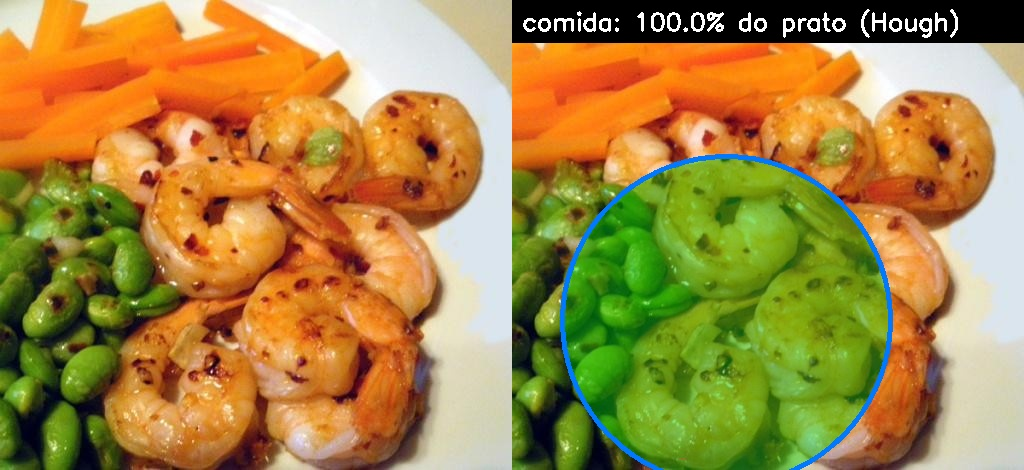
\includegraphics[width=\textwidth]{figuras/exemplo_pipeline.jpg}
  \caption{Saída do pipeline em imagem de validação: original (esquerda) e resultado
  (direita), com máscara de comida, círculo de Hough e percentual calculado. Nesta execução de
  validação o modelo havia sido treinado por apenas 2 épocas em 40 imagens, com limiar de
  confiança reduzido; a imagem, em close, não contém a borda completa do prato, e o círculo
  encontrado não corresponde a ela --- caso discutido na Seção~\ref{sec:limitacoes}.}
  \label{fig:pipeline}
\end{figure}

\subsection{Métricas do treinamento}

O treinamento completo (50 épocas sobre as 4.983 imagens de treino) produz as métricas padrão
de segmentação reportadas pelo framework Ultralytics sobre o conjunto de validação (2.135
imagens): precisão, revocação e mAP (\emph{mean Average Precision}) para caixas e máscaras.
Os valores finais devem ser extraídos de \texttt{runs/food-seg/results.csv} ao término do
treinamento e estão resumidos na Tabela~\ref{tab:metricas}.

\begin{table}[H]
  \centering
  \caption{Métricas de validação após o treinamento completo (máscaras).}
  \label{tab:metricas}
  \begin{tabular}{lc}
    \toprule
    Métrica (máscara, classe \texttt{food}) & Valor \\
    \midrule
    Precisão ($P$)          & --- \\
    Revocação ($R$)         & --- \\
    mAP@50                  & --- \\
    mAP@50--95              & --- \\
    \bottomrule
  \end{tabular}
\end{table}

\subsection{Limitações}
\label{sec:limitacoes}

\begin{itemize}
  \item \textbf{Medida bidimensional}: a projeção da comida no plano da imagem não captura
        altura; porções empilhadas e camadas finas com a mesma projeção resultam no mesmo
        $Q$. Uma extensão natural seria estimar volume com visão estéreo ou luz estruturada;
  \item \textbf{Hipótese de prato circular}: a transformada de Hough pressupõe borda circular
        razoavelmente completa no quadro. Muitas imagens do FoodSeg103 são \emph{closes} sem a
        borda do prato, situação em que o sistema recua para a imagem inteira como referência
        --- o resultado permanece bem definido, mas perde a normalização pelo prato;
  \item \textbf{Domínio do dataset}: o FoodSeg103 contém fotografias de refeições variadas;
        cenários muito diferentes (iluminação extrema, pratos coloridos ou estampados) podem
        degradar tanto a segmentação quanto a detecção do prato.
\end{itemize}

% ---------------------------------------------------------------- 5
\section{Conclusão}

Este trabalho demonstrou a construção completa, em máquina local, de um sistema de estimativa
de quantidade de comida em pratos a partir de fotografias. A solução integra, de forma
complementar, aprendizado profundo (segmentação de instâncias com YOLOv8n-seg ajustado no
FoodSeg103) e técnicas clássicas de processamento de sinais bidimensionais (filtro de mediana,
detecção de bordas por gradiente e transformada de Hough circular), ilustrando na prática como
os conceitos da disciplina --- convolução 2D, filtragem não linear, gradiente e detecção
paramétrica de formas --- permanecem centrais mesmo em pipelines modernos de visão
computacional: as próprias camadas da rede neural são bancos de filtros convolucionais cujos
coeficientes são aprendidos dos dados.

Como trabalhos futuros, destacam-se a estimativa de volume (3D) da porção, o suporte a pratos
não circulares via segmentação do prato pela própria rede e a validação quantitativa da medida
$Q$ contra pesagens reais.

% ---------------------------------------------------------------- REFS
\begin{thebibliography}{9}

\bibitem{gonzalez}
R.~C. Gonzalez e R.~E. Woods, \emph{Digital Image Processing}, 4.~ed. Pearson, 2018.

\bibitem{canny}
J.~Canny, ``A computational approach to edge detection'', \emph{IEEE Transactions on Pattern
Analysis and Machine Intelligence}, vol. PAMI-8, n.~6, pp. 679--698, 1986.

\bibitem{hough}
R.~O. Duda e P.~E. Hart, ``Use of the Hough transformation to detect lines and curves in
pictures'', \emph{Communications of the ACM}, vol.~15, n.~1, pp. 11--15, 1972.

\bibitem{foodseg103}
X.~Wu \emph{et al.}, ``A large-scale benchmark for food image segmentation'', em
\emph{Proceedings of the 29th ACM International Conference on Multimedia}, 2021, pp. 506--515.

\bibitem{yolov8}
G.~Jocher, A.~Chaurasia e J.~Qiu, ``Ultralytics YOLOv8'', 2023. Disponível em:
\url{https://github.com/ultralytics/ultralytics}.

\bibitem{opencv}
G.~Bradski, ``The OpenCV library'', \emph{Dr. Dobb's Journal of Software Tools}, 2000.

\end{thebibliography}

\end{document}
